%
\documentclass[
  notoc % Suppress Tufte style table of contents.
]{tufte-book}

% Required Tufte packages.
\usepackage{changepage} % or changepage
\usepackage{fancyhdr}
\usepackage{fontenc}
\usepackage{geometry}
\usepackage{hyperref}
\usepackage{natbib}
\usepackage{bibentry}
\usepackage{optparams}
\usepackage{paralist}
\usepackage{placeins}
\usepackage{ragged2e}
\usepackage{setspace}
\usepackage{textcase}
\usepackage{textcomp}
\usepackage{titlesec}
\usepackage{titletoc}
\usepackage{xcolor}
\usepackage{xifthen}
\usepackage{morefloats}

\geometry{paperheight=10in,paperwidth=7in,marginparwidth=30mm,marginparsep=2mm,bindingoffset=10mm,top=10mm,inner=8mm,outer=8mm,bottom=16mm,includehead,includemp}

% Tufte vs. Pandoc workaround.
% Issue: https://github.com/Tufte-LaTeX/tufte-latex/issues/64.
\renewcommand\allcapsspacing[1]{{\addfontfeature{LetterSpace=15}#1}}
\renewcommand\smallcapsspacing[1]{{\addfontfeature{LetterSpace=10}#1}}

% \setmainfont{TeX Gyre Pagella}
\usepackage[utf8]{inputenc}
\usepackage[T1]{fontenc}
\setmainfont{texgyrepagella}[
  Extension = .otf,
  UprightFont = *-regular,
  BoldFont = *-bold,
  ItalicFont = *-italic,
  BoldItalicFont = *-bolditalic,
]

\usepackage{fontspec}
\setmonofont{JuliaMono-Medium.ttf}[
    % Do not remove the trailing forward slash.
    Path = /home/yidai/.julia/artifacts/45f34ceb7f1b7b67949715de56b123afeaa72e47/juliamono-0.045/,
    Contextuals = Alternate,
    Ligatures = NoCommon
]

\newfontface\JuliaMonoRegular{JuliaMono-Regular.ttf}[
    Path = /home/yidai/.julia/artifacts/45f34ceb7f1b7b67949715de56b123afeaa72e47/juliamono-0.045/,
    Contextuals = Alternate,
    Ligatures = NoCommon
]

\newfontface\JuliaMonoBold{JuliaMono-Bold.ttf}[
    Path = /home/yidai/.julia/artifacts/45f34ceb7f1b7b67949715de56b123afeaa72e47/juliamono-0.045/,
    Contextuals = Alternate,
    Ligatures = NoCommon
]



\usepackage{graphicx}
\makeatletter
\def\maxwidth{\ifdim\Gin@nat@width>\linewidth\linewidth\else\Gin@nat@width\fi}
\def\maxheight{\ifdim\Gin@nat@height>\textheight\textheight\else\Gin@nat@height\fi}
\makeatother
% Scale images if necessary, so that they will not overflow the page
% margins by default, and it is still possible to overwrite the defaults
% using explicit options in \includegraphics[width, height, ...]{}
\setkeys{Gin}{width=\maxwidth,height=\maxheight,keepaspectratio}
\DeclareRobustCommand{\href}[2]{#2\footnote{\url{#1}}}

\usepackage{float}
\floatplacement{figure}{H}

% Listings Julia syntax definition.
\input{/home/yidai/.julia/packages/Books/odNoe/defaults/julia_listings.tex}

% Unicode support.
\input{/home/yidai/.julia/packages/Books/odNoe/defaults/julia_listings_unicode.tex}

% Used by Pandoc.
\providecommand{\tightlist}{%
  \setlength{\itemsep}{0pt}\setlength{\parskip}{0pt}
}
\newcommand{\passthrough}[1]{#1}

\usepackage{longtable}
\usepackage{booktabs}
\usepackage{array}

% Source: Wandmalfarbe/pandoc-latex-template.

\definecolor{linkblue}{HTML}{117af2}
\usepackage{hyperref}
\hypersetup{
  colorlinks,
  citecolor=linkblue,
  linkcolor=linkblue,
  urlcolor=linkblue,
  linktoc=page, % Avoid Table of Contents being nearly completely blue.
  pdftitle={Scientific Computing for Physicist},
  pdfauthor={Yu-Sheng Zhao; Yi-Dai Zhang; Jin-Guo Liu},
  pdflang={en-US},
  breaklinks=true,
  pdfcreator={LaTeX via Pandoc}%
}
\urlstyle{same} % disable monospaced font for URLs

\title{Scientific Computing for Physicist}
\author{\noindent{Yu-Sheng Zhao}\\[3mm] \noindent{Yi-Dai
Zhang}\\[3mm] \noindent{Jin-Guo Liu}\\[3mm] }
\date{}

% Re-enable section numbering which was disabled by tufte.
\setcounter{secnumdepth}{2}

% Fix captions for longtable.
% Thanks to David Carlisle at https://tex.stackexchange.com/a/183344/92217.
\makeatletter
\def\LT@makecaption#1#2#3{%
  \noalign{\smash{\hbox{\kern\textwidth\rlap{\kern\marginparsep
  \parbox[t]{\marginparwidth}{\vspace{12pt}%
\@tufte@caption@font \@tufte@caption@justification \noindent
   #1{#2: }\ignorespaces #3}}}}}}
\makeatother

% Doesn't seem to do anything.
\usepackage{float}
\floatplacement{figure}{H}
\floatplacement{table}{H}

% Reduce large spacing around sections.
\titlespacing*{\chapter}{0pt}{5pt}{20pt}
\titlespacing*{\section}{0pt}{2.5ex plus 1ex minus .2ex}{1.3ex plus .2ex}
\titlespacing*{\subsection}{0pt}{1.75ex plus 1ex minus .2ex}{1.0ex plus.2ex}

\titleformat{\chapter}%
  [hang]% shape
  {\normalfont\huge\itshape}% format applied to label+text
  {\huge\thechapter}% label
  {1em}% horizontal separation between label and title body
  {}% before the title body
  []% after the title body

% Reduce spacing in table of contents.
\usepackage{etoolbox}
\makeatletter
\pretocmd{\chapter}{\addtocontents{toc}{\protect\addvspace{-3\p@}}}{}{}
\pretocmd{\section}{\addtocontents{toc}{\protect\addvspace{-4\p@}}}{}{}
\pretocmd{\subsection}{\addtocontents{toc}{\protect\addvspace{-5\p@}}}{}{}
\makeatother

% Long texts are harder to read than tables.
% Therefore, we can reduce the font size of the table.
\AtBeginEnvironment{longtable}{\footnotesize}

% Some space between paragraphs is necessary because code blocks can output single line paragraphs.
\setlength\parskip{1em plus 0.1em minus 0.2em}

% For justified text.
\usepackage{ragged2e}

% tufte-book disables subsubsections by default.
% Got this definition back via `\show\subsubsection`.

\usepackage{amsfonts}
\usepackage{amssymb}
\usepackage{amsmath}
\usepackage{unicode-math}

% URL line breaks.
\usepackage{xurl}

% Probably doesn't hurt.
\usepackage{marginfix}




\begin{document}

\makeatletter
\thispagestyle{empty}
\vfill
{\Huge\bf
\noindent
\@title
}\\[1in]
{\Large
\noindent
\@author
}
\makeatother

\makeatletter
\newpage
\thispagestyle{empty}
\vfill
{\noindent
\begin{tabular}{l} Yu-Sheng Zhao\\ Hong-Kong University of Science and Technology (Guangzhou)\\ \\ Yi-Dai Zhang\\ Hong-Kong University of Science and Technology (Guangzhou)\\ \\ Jin-Guo Liu\\ Hong-Kong University of Science and Technology (Guangzhou)\\ \\ \end{tabular}
}
\vfill
{\small
\url{https://book.jinguo-group.science}

Version: 2024-02-18

Creative Commons Attribution-NonCommercial-ShareAlike 4.0 International
}
\makeatother


% Don't remove this or authors will show up in header of every page.
\frontmatter
\mainmatter
\fancyfoot[C]{\url{https://github.com/johndoe/Book.jl}}

\setcounter{tocdepth}{1}
\tableofcontents

% Justify text.
\justifying

% parindent seems to be set from within another class too.
% it is really not useful here because it will also indent lines directly after
% code blocks. Which most of the times not useful.
\setlength{\parindent}{0pt}

\hypertarget{sec:open-source-dev-toolchains}{%
\chapter{Becoming an Open-Source
Developer}\label{sec:open-source-dev-toolchains}}

This section focuses on understanding the open source workflow, which is
the foundation of scientific computing. Along the way, we will introduce
to you our recommended tools for accomplishing each task.

\hypertarget{get-a-terminal}{%
\section{Get a Terminal!}\label{get-a-terminal}}

You need to get a working terminal to follow the instructions in this
book, because everyone who thinks he is cool uses a terminal.

\hypertarget{sec:linux}{%
\subsection{Linux operating system}\label{sec:linux}}

Using Linux is the most straight-forward way to get a terminal. Just
like Windows, IOS, and Mac OS, Linux is an operating system. In fact,
Android, one of the most popular platforms on the planet, is powered by
the Linux operating system. It is free to use,
\href{https://opensource.com/resources/what-open-source}{open source},
widely used on clusters and good at automating your works. Linux kernel,
Linux operating system and Linux distribution are different concepts.
A~\textbf{Linux distribution} is
an~\href{https://en.wikipedia.org/wiki/Operating_system}{operating
system}~made from a software collection that includes
the~\href{https://en.wikipedia.org/wiki/Linux_kernel}{Linux kernel}~and,
often,
a~\href{https://en.wikipedia.org/wiki/Package_management_system}{package
management system} The Linux kernel is started
by~\href{https://en.wikipedia.org/wiki/Linus_Torvalds}{Linus Torvalds}
in 1991.

The Linux distribution we will use for demoing and live-coding is the
\href{https://ubuntu.com/desktop}{Ubuntu} distribution of the
\href{https://en.wikipedia.org/wiki/Linux}{Linux} operating system.

\hypertarget{sec:shell}{%
\subsection{Shell (or Terminal)}\label{sec:shell}}

Although you can use a \textbf{graphical user interface} (GUI) to
interact with your Linux distribution, you will find that the
\textbf{command line interface} (CLI) is more efficient and powerful.
The CLI is also known as the \textbf{shell} or \textbf{terminal}.

The shell is a program that takes commands from the keyboard and gives
them to the operating system to perform. \href{https://zsh.org/}{Zsh}
and \href{https://gnu.org/software/bash/}{Bash} are all shell
interpreters used in the Linux operating systems.

\textbf{Bash}(Bourne-Again SHell) is the default shell on most Linux
distributions. It is backward-compatible with the original Bourne shell
and includes many additional features, such as command-line editing, job
control, and shell scripting capabilities. Bash is widely used as it is
both easy to use and has a large user community, resulting in a plethora
of available resources (tutorials, scripts, etc.) online.

\textbf{Zsh}(Z shell) is an extended version of the shell, with a more
powerful command-line editing and completion system. It includes
features like spelling correction and tab-completion, and it also
supports plugins and themes. Zsh is commonly used by power users who
require more productivity and efficiency from their command-line
interface.

We will be using \passthrough{\lstinline!Bash!} during this course. In
Ubuntu, one can use \passthrough{\lstinline!Ctrl!} +
\passthrough{\lstinline!Alt!} + \passthrough{\lstinline!T!} to open a
\passthrough{\lstinline!Bash!} shell. In a
\passthrough{\lstinline!Bash!} shell, we use
\passthrough{\lstinline!man command\_name!} to get help information
related to a command, use \passthrough{\lstinline!CTRL-C!} to break a
program and \passthrough{\lstinline!CTRL-D!} to exit a shell or an REPL.

The following is a short list of bash commands that will be used
frequently in this book.

\begin{lstlisting}
man     # an interface to the system reference manuals

ls      # list directory contents
cd      # change directory
mkdir   # make directories
rm      # remove files or directories
pwd     # print name of current/working directory

echo    # display a line of text
cat     # concatenate files and print on the standard output

alias   # create an alias for a command

lscpu   # display information about the CPU architecture
lsmem   # list the ranges of available memory with their online status

top     # display Linux processes
ssh     # the OpenSSH remote login client
vim     # Vi IMproved, a programmer's text editor
git     # the stupid content tracker

tar     # an archiving utility
\end{lstlisting}

The power and convinence provided by \passthrough{\lstinline!Bash!} far
exceeds what this list can express.

\textbf{Resources}

\begin{itemize}
\tightlist
\item
  \href{https://missing.csail.mit.edu/2020/shell-tools/}{MIT Open
  course: Missing semester}
\item
  \href{https://www.learnshell.org/}{Learn Bash Shell}
\item
  \href{https://www.shellscript.sh/}{Shell Scripting Tutorial}
\item
  \href{https://devhints.io/bash}{Bash scripting cheatsheet}
\end{itemize}

\hypertarget{sec:editor}{%
\subsection{Vim Editor}\label{sec:editor}}

In order to write code, you need an editor. There are many editors
available for you to choose from. We recommend the following editors for
different purposes.

\passthrough{\lstinline!Vim!} is a highly configurable and light-weight
text editor built to enable efficient text editing. It can be found in
any Linux distribution, with or without a graphical user interface. This
feature makes it especially useful and essential to master when you are
dealing with servers often. \passthrough{\lstinline!Vim!} is known for
its modal editing, a design that allows the user to switch between
different modes of operation, each tailored for specific tasks. The
primary modes include \textbf{Normal Mode}, used for navigating and
manipulating text; \textbf{Insert Mode}, where users can insert text as
in conventional text editors; \textbf{Visual Mode}, enabling text
selection for operations like cutting, copying, or formatting;
\textbf{Command Mode}, where users input commands for tasks like saving
files or searching; and \textbf{Replace Mode}, which is used to
overwrite existing text. This modal approach in Vim optimizes efficiency
by separating the tasks of editing and navigating, allowing for quicker
and more precise text manipulation. Users can seamlessly switch between
these modes, leveraging the unique capabilities of each to enhance their
text editing workflow.

A few commands are listed below to get you started with
\passthrough{\lstinline!Vim!}.

\begin{lstlisting}
i       # input
:w      # write
:q      # quit
:q!     # force quit without saving

u       # undo
CTRL-R  # redo
\end{lstlisting}

All the commands must be executed in the \textbf{command mode}. If you
are currently in the input mode, you can alway type
\passthrough{\lstinline!ESC!} to go back to the command mode.

To learn more about Vim, please check this
\href{https://missing.csail.mit.edu/2020/editors/}{lecture}.

As an example, to edit the config file
\passthrough{\lstinline!\~/.ssh/config!} just type
\passthrough{\lstinline!vim \~/.ssh/config!}.

\hypertarget{sec:ssh}{%
\subsection{SSH}\label{sec:ssh}}

The programmer may not always have access to a powerful machine for both
running and development of his code. He/she may ``borrow'' the power of
a remote machine with the help of \passthrough{\lstinline!ssh!} command.
The underlying work force of \passthrough{\lstinline!ssh!} is
\textbf{Secure Shell}. \textbf{Secure Shell} is a network protocol that
allows the user to take command of a remote server securely. After
establishing the \textbf{Secure Shell} connection, the user can take
command of a server via sending it shell commands.

With a host name (the IP of the target machine to login) and a user
name, one can use the following command to login,

\begin{lstlisting}[language=bash]
ssh <username>@<hostname>
\end{lstlisting}

where \passthrough{\lstinline!<username>!} is the user name and
\passthrough{\lstinline!<hostname>!} is the host name or IP of the
target machine. You will get logged in after inputting the password.

\textbf{Tips to make your life easier}

It will be tedious to type the host name and user name everytime you
want to login to the remote machine. You can setup the
\passthrough{\lstinline!\~/.ssh/config!} file to make your life easier.
The following is an example of the
\passthrough{\lstinline!\~/.ssh/config!} file.

\begin{lstlisting}
Host amat5315
  HostName <hostname>
  User <username>
\end{lstlisting}

where \passthrough{\lstinline!amat5315!} is the alias of the host. After
setting up the \passthrough{\lstinline!\~/.ssh/config!}, you can login
to the remote machine by typing

\begin{lstlisting}[language=bash]
ssh amat5315
\end{lstlisting}

If you want to avoid typing the password everytime you login, you can
use the command

\begin{lstlisting}[language=bash]
ssh-keygen
\end{lstlisting}

to generate a pair of public and private keys, which will be stored in
the \passthrough{\lstinline!\~/.ssh!} folder on the local machine. After
setting up the keys, you can copy the public key to the remote machine
by typing

\begin{lstlisting}[language=bash]
ssh-copy-id amat5315
\end{lstlisting}

Try connecting to the remote machine again, you will find that you don't
need to type the password anymore.

\textbf{How does SSH key pair work?} The SSH key pair is a pair of
asymmetric keys, one is the public key and the other is the private key.
In the above example, the public key is uploaded to the remote machine
and the private key is stored on the local machine. The public key can
be shared with anyone, but the private key must be kept secret.

To connect to a server, the server needs to know that you are the one
who with the right to access it. To do so, the server will need to check
if you have the private key that corresponds to the public key stored on
the server. If you have the private key, you will be granted access to
the server.

The secret of the SSH key pair is that \textbf{the public key can be
used to encrypt a message that can only be decrypted by the private
key}, i.e.~the public key is more like a lock and the private key is the
key to unlock the lock. This is the foundation of the SSH protocol. So
server can send you a message encrypted by your public key, and only you
can decrypt it with your private key. This is how the server knows that
you are the one who has the private key without actually sending the
private key to the server.

\hypertarget{sec:version-control}{%
\section{Code MUST be Maintained: Version
Control}\label{sec:version-control}}

Maintaining a software project is not easy. You may encounter the
following problems:

\begin{itemize}
\tightlist
\item
  New code breaks an existing feature
\item
  Conflicts between two changes
\item
  No working code!
\item
  Bug fixes at a wrong version
\item
  Code lost
\end{itemize}

A crucial part of maintaining an open-source software is
\textbf{version-control}. In the following, we will introduce the best
tool for doing version-control: \textbf{Git}.

\hypertarget{what-is-a-repo}{%
\subsection{What is a repo?}\label{what-is-a-repo}}

A repository, also known as a repo, is basically a directory where your
project lives and git keeps track of your file's history.

\begin{itemize}
\tightlist
\item
  You start with a working directory, then use
  \passthrough{\lstinline!git init!} to make it a git repository.
\item
  You can use \passthrough{\lstinline!git add!} to add files to the
  staging area, and use \passthrough{\lstinline!git commit!} to commit
  the changes to the repository.
\item
  You can use \passthrough{\lstinline!git checkout!} to switch between
  commits.
\item
  You can use \passthrough{\lstinline!git diff!} to see the changes
  between commits.
\item
  You can use \passthrough{\lstinline!git reset!} to reset the current
  HEAD to the specified state.
\item
  You can use \passthrough{\lstinline!git status!} to see the status of
  the working directory, staging area, and repository.
\item
  You can use \passthrough{\lstinline!git log!} to see the history of
  commits.
\end{itemize}

\hypertarget{working-with-remote-repositories}{%
\subsection{Working with remote
repositories}\label{working-with-remote-repositories}}

Now that you have configuration all setup, we will get you familiarized
with a few concepts. In Git terminology, \textbf{Remote} refers to a
repository that is located on a server or another computer, rather than
the user's local machine. It's a version of the repository that is used
by teams to collaborate on a project. Remote repositories can be
accessed and manipulated through Git commands, allowing users to push
changes or fetch changes made by others. Remote repositories can be
hosted on Git hosting services like GitHub, GitLab, or Bitbucket, or set
up on a personal server. Multiple users can access and modify the same
remote repository, making it easy for teams to work on a project
together.

\begin{itemize}
\tightlist
\item
  You can use
  \passthrough{\lstinline!git remote add <remote-name> <url>!} to add a
  remote repository.
\item
  You can use \passthrough{\lstinline!git push <remote-name> <branch>!}
  to push commits to a remote repository.
\item
  You can use \passthrough{\lstinline!git pull <remote-name> <branch>!}
  to fetch from and integrate with another repo or a local branch.
\end{itemize}

\hypertarget{developing-a-feature-safely}{%
\subsection{Developing a feature
safely}\label{developing-a-feature-safely}}

A branch in Git is a lightweight pointer to a specific commit. It allows
developers to work on new features or make changes to the codebase
without affecting the main codebase. Branches are created and can be
switched between easily, and changes made in one branch do not affect
other branches.

To create a new branch in Git, you can use the command
\passthrough{\lstinline!git branch <branch\_name>!}. This creates a new
branch but does not switch to it, so you will be working in the same
branch until you use the command
\passthrough{\lstinline!git checkout <branch\_name>!} to switch to the
new branch. Alternatively, you can use the command
\passthrough{\lstinline!git checkout -b <branch\_name>!} to create and
switch to the new branch at the same time.

To end a branch, you can use the command
\passthrough{\lstinline!git branch -d <branch\_name>!}. This deletes the
specified branch, but only if it has been fully merged into the main
branch. If you want to delete a branch whether it has been fully merged
or not, you can use the command
\passthrough{\lstinline!git branch -D <branch\_name>!}. It's important
to note that once a branch has been deleted, you cannot restore its
commit history.

\hypertarget{example-workflow}{%
\subsection{Example Workflow}\label{example-workflow}}

Here are two example workflows managing your project with git.

Example 1: develop a new feature
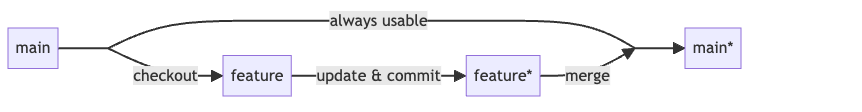
\includegraphics{./assets/images/newfeature.png}

Example 2: develop two features
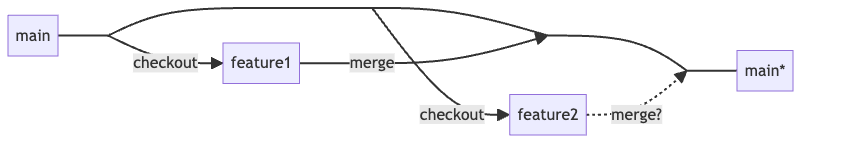
\includegraphics{./assets/images/twofeatures.png}

\hypertarget{cheatsheet-and-resources-for-git-and-github}{%
\subsection{Cheatsheet and Resources for Git and
Github}\label{cheatsheet-and-resources-for-git-and-github}}

It is not possible to cover all of the feature of git. We will list a
few useful commands and resources for git learning.

\begin{lstlisting}
# global config
git config  # Get and set repository or global options

# initialize a repo
git init    # Create an empty Git repo or reinitialize an existing one
git clone   # Clone repository into new directory

# info
git status  # Show the working tree status
git log     # Show commit logs
git diff    # Show changes between commits, commit and working tree, etc

# work on a branch
git add     # Add file contents to the index
git rm      # Remove files from the working tree and from the index
git commit  # Record changes to the repository
git reset   # Reset current HEAD to the specified state

# branch manipulation
git checkout # Switch branches or restore working tree files
git branch  # List, create, or delete branches
git merge   # Join two or more development histories together

# remote synchronization
git remote  # Manage set of tracked repositories
git pull  # Fetch from and integrate with another repo or a local branch
git fetch   # Download objects and refs from another repository
git push    # Update remote refs along with associated objects
\end{lstlisting}

A more detailed introduction could be found in this
\href{https://missing.csail.mit.edu/2020/version-control/}{lecture}.

\hypertarget{resources}{%
\subsection{Resources}\label{resources}}

\begin{itemize}
\tightlist
\item
  \href{https://www.learnshell.org/}{Learn Bash Shell}
\item
  \href{https://learngitbranching.js.org/}{Learn Git}
\item
  \href{https://githubtraining.github.io/training-manual/book.pdf}{Github
  Manual}
\item
  \href{https://docs.github.com/en/get-started/quickstart/create-a-repo}{How
  to create a new github repo}
\item
  \href{https://docs.github.com/en/pull-requests/collaborating-with-pull-requests/proposing-changes-to-your-work-with-pull-requests/creating-a-pull-request}{How
  to create a pull request}
\item
  \href{https://www.markdowntutorial.com/}{Markdown Tutorial}
\item
  MIT online course \href{https://missing.csail.mit.edu/2020/}{missing
  semester}.
\item
  \href{https://learngitbranching.js.org/?locale=zh_CN}{Learn Git with
  Game}
\item
  \href{https://dev.to/lydiahallie/cs-visualized-useful-git-commands-37p1}{Command
  Visualization}
\item
  \href{https://ohshitgit.com/}{Git Panic}
\end{itemize}

\hypertarget{sec:ci-cd}{%
\section{Code MUST be Tested!}\label{sec:ci-cd}}

In terms of scientific computing, accuracy of your result is most
certainly more important than anything else. To ensure the correctness
of the code, we employ two methods: \textbf{Unit Testing} and
\textbf{CI/CD}.

\hypertarget{unit-test}{%
\subsection{Unit Test}\label{unit-test}}

Unit tests are typically
\href{https://en.wikipedia.org/wiki/Automated_test}{automated tests}
written and run by
\href{https://en.wikipedia.org/wiki/Software_developer}{software
developers} to ensure that a section of an application (known as the
``unit'') meets its
\href{https://en.wikipedia.org/wiki/Software_design}{design} and behaves
as intended. In \passthrough{\lstinline!Julia!}, there exists a helpful
module called \href{https://docs.julialang.org/en/v1/stdlib/Test/}{Test}
to help you do Unit Testing.

\hypertarget{cicd}{%
\subsection{CI/CD}\label{cicd}}

Continuous Integration (CI) and Continuous Deployment (CD) are
fundamental practices in modern software development aimed at enhancing
the efficiency and quality of software production. CI is the process of
automatically integrating code changes from multiple contributors into a
single software project. This involves frequent code version submissions
to a shared repository, where automated builds and tests are run. The
primary goal of CI is to identify and address conflicts and bugs early,
ensuring that the main codebase remains stable and release-ready at all
times.

On the other hand, CD extends CI by automating the delivery of
applications to selected infrastructure environments. This can range
from automated testing stages to full-scale production deployments. The
main advantage of CD is its ability to release new changes to customers
quickly and sustainably. It enables a more rapid feedback loop, where
improvements and fixes are delivered faster to end-users.

Together, CI/CD embody a culture of continuous improvement and
efficiency, where software quality is enhanced, and development cycles
are shortened. This not only reduces the time and cost of software
development but also allows teams to respond more swiftly to market
changes and customer needs, maintaining a competitive edge in the
fast-paced tech world.

\hypertarget{learn-to-collaborate}{%
\section{Learn to Collaborate}\label{learn-to-collaborate}}

\begin{itemize}
\tightlist
\item
  You can open an issue on
  GitHub/\href{https://en.wikipedia.org/wiki/GitLab}{GitLab} to report a
  bug or request a feature.
\item
  You can create
  \href{https://docs.github.com/en/pull-requests/collaborating-with-pull-requests/proposing-changes-to-your-work-with-pull-requests/creating-a-pull-request}{a
  pull request} on GitHub/GitLab to propose changes to a repository and
  discuss them with others.
\end{itemize}

Example: collaborate with others
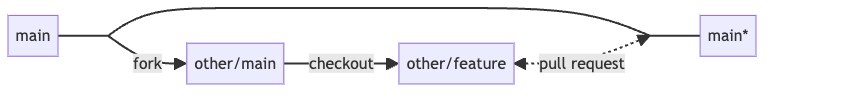
\includegraphics{./assets/images/collab.png}

\hypertarget{share-your-code}{%
\section{Share Your Code}\label{share-your-code}}

Now that you have an amazing package, it's time to make it available to
the public. Before that, there is one final task to be done which is to
choose a license.

\begin{itemize}
\item
  GNU's Not Unix! (GNU) (1983 by Richard Stallman)

  Its goal is to give computer users freedom and control in their use of
  their computers
  and~\href{https://en.wikipedia.org/wiki/Computer_hardware}{computing
  devices}~by collaboratively developing and publishing software that
  gives everyone the rights to freely run the software, copy and
  distribute it, study it, and modify it. GNU software grants these
  rights in
  its~\href{https://en.wikipedia.org/wiki/GNU_General_Public_License}{license}.
\item
  The problem of GPL Lisense: The GPL and licenses modeled on it impose
  the restriction that source code must be distributed or made available
  for all works that are derivatives of the GNU copyrighted code.

  Case study:
  \href{https://www.notion.so/Wiki-53dd9dafd57b40f6b253d6605667a472}{Free
  Software fundation v.s. Cisco Systems}

  Modern Licenses are:
  \href{https://en.wikipedia.org/wiki/MIT_License}{MIT} and
  \href{https://en.wikipedia.org/wiki/Apache_License}{Apache}.
\end{itemize}

\hypertarget{sec:julia}{%
\chapter{Julia}\label{sec:julia}}

\passthrough{\lstinline!Julia!} is a high-level, high-performance,
dynamic programming language. From the designing stage,
\passthrough{\lstinline!Julia!} is intended to address the needs of
high-performance numerical analysis and computational science, without
the typical need of separate compilation to be fast, while also being
effective for general-purpose programming, web use or as a specification
language. \passthrough{\lstinline!Julia!} is also a free and open-source
language, with a \href{https://julialang.org/community/}{large
community} and a \href{https://juliahub.com/}{rich ecosystem}.

We will devlve deeper into \passthrough{\lstinline!Julia!} later in the
chapter. For now, we will just install \passthrough{\lstinline!Julia!}
and setup the environment.

\hypertarget{sec:setup}{%
\section{Setup Julia}\label{sec:setup}}

\hypertarget{step-1-installing-julia}{%
\subsection{Step 1: Installing Julia}\label{step-1-installing-julia}}

For Linux/Mac users, please open a terminal and type the following
command to install \href{https://julialang.org/}{Julia} with
\href{https://github.com/JuliaLang/juliaup}{juliaup}.
\passthrough{\lstinline!Juliaup!} is a tool to manage Julia versions and
installations. It allows you to install multiple versions of Julia and
switch between them easily.

\begin{lstlisting}[language=bash]
curl -fsSL https://install.julialang.org | sh # Linux and macOS
\end{lstlisting}

For Windows users, please open execute the following command in a
\passthrough{\lstinline!cmd!},

\begin{lstlisting}
winget install julia -s msstore # Windows
\end{lstlisting}

You can also install Juliaup directly from
\href{https://www.microsoft.com/store/apps/9NJNWW8PVKMN}{Windows Store}.

\hypertarget{for-users-suffering-from-the-slow-download-speed}{%
\subsection{For users suffering from the slow download
speed}\label{for-users-suffering-from-the-slow-download-speed}}

Network connectivity can be an issue for some users, especially for
those who are in China. You may need to specify another server for
installing Juliaup and Julia packages. To do so, execute the following
command in your terminal before running the script above.

\textbf{Linux and macOS}

\begin{lstlisting}[language=bash]
export JULIAUP_SERVER=https://mirror.nju.edu.cn/julia-releases/ # Linux & macOS
export JULIA_PKG_SERVER=https://mirrors.nju.edu.cn/julia
\end{lstlisting}

\textbf{Windows}

\begin{lstlisting}
$env:JULIAUP_SERVER="https://mirror.nju.edu.cn/julia-releases/" # Windows
$env:JULIA_PKG_SERVER="https://mirrors.nju.edu.cn/julia"
\end{lstlisting}

An alternative approach is downloading the corresponding Julia binary
from the \href{https://mirror.nju.edu.cn/julia-releases/}{Nanjing
university mirror website}. After installing the binary, please set the
Julia binary path properly if you want to start a Julia REPL from a
terminal, check this
\href{https://julialang.org/downloads/platform/}{manual page} to learn
more.

\hypertarget{installing-julia}{%
\subsection{Installing Julia}\label{installing-julia}}

To verify that Julia is installed, please open a \textbf{new} terminal
and run the following command in your terminal.
\passthrough{\lstinline!bash   julia!} - It should start a Julia
REPL(Read-Eval-Print-Loop) session like this - If you wish to install a
specific version of Julia, please refer to the
\href{https://github.com/JuliaLang/juliaup}{documentation}.

\hypertarget{step-2-package-management}{%
\subsection{Step 2: Package
Management}\label{step-2-package-management}}

\begin{itemize}
\tightlist
\item
  \passthrough{\lstinline!Julia!} has a mature eco-system for scientific
  computing.
\item
  \passthrough{\lstinline!Pkg!} is the built-in package manager for
  Julia.
\item
  To enter the package manager, press \passthrough{\lstinline!]!} in the
  REPL.
  \includegraphics{https://github.com/exAClior/QMBCTutorial/blob/ys/julia-tutorial/notebooks/resources/scripts/Packages.gif?raw=true}
\item
  The environment is indicated by the \passthrough{\lstinline!(@v1.9)!}.
\item
  To add a package, type \passthrough{\lstinline!add <package name>!}.
\item
  To exit the package manager press \passthrough{\lstinline!backspace!}
  key
\item
  \href{https://pkgdocs.julialang.org/v1/managing-packages/}{Read More}
\end{itemize}

\hypertarget{step-3.-configure-the-startup-file}{%
\subsection{Step 3. Configure the startup
file}\label{step-3.-configure-the-startup-file}}

First create a new file
\passthrough{\lstinline!\~/.julia/config/startup.jl!} by executing the
following commands

\passthrough{\lstinline!mkdir -r \~/.julia/config!}
\passthrough{\lstinline!touch \~/.julia/config/startup.jl!}

You could open the file with your favourite editor and add the following
content

\begin{lstlisting}
try
    using Revise
catch e
    @warn "fail to load Revise."
end
\end{lstlisting}

The contents in the startup file is executed immediately after you open
a new Julia session.

Then you need to install
\href{https://github.com/timholy/Revise.jl}{Revise}, which is an Julia
package that can greatly improve the using experience of Julia. To
install \passthrough{\lstinline!Revise!}, open Julia REPL and type

\begin{lstlisting}
julia> using Pkg; Pkg.add("Revise")
\end{lstlisting}

If you don't know about \passthrough{\lstinline!startup.jl!} and where
to find it,
\href{https://docs.julialang.org/en/v1/manual/command-line-interface/\#Startup-file}{here}
is a good place for further information.

\hypertarget{more-packages}{%
\subsection{More Packages}\label{more-packages}}

\begin{itemize}
\tightlist
\item
  You may find more Julia packages \href{https://juliahub.com/}{here}.
\end{itemize}

As a final step, please verify your Julia configuration by openning a
Julia REPL and type

\begin{lstlisting}
julia> versioninfo()
Julia Version 1.9.2
Commit e4ee485e909 (2023-07-05 09:39 UTC)
Platform Info:
  OS: macOS (arm64-apple-darwin22.4.0)
  CPU: 10 × Apple M2 Pro
  WORD_SIZE: 64
  LIBM: libopenlibm
  LLVM: libLLVM-14.0.6 (ORCJIT, apple-m1)
  Threads: 1 on 6 virtual cores
Environment:
  JULIA_NUM_THREADS = 1
  JULIA_PROJECT = @.
  JULIA_PKG_SERVER = http://cn-southeast.pkg.juliacn.com/ 
\end{lstlisting}

\hypertarget{step-4.-download-an-editor-vscode}{%
\subsection{Step 4. Download an editor:
VSCode}\label{step-4.-download-an-editor-vscode}}

Install VSCode by downloading the correct binary for your platform from
\href{https://code.visualstudio.com/download}{here}. Open VSCode and
open the \passthrough{\lstinline!Extensions!} tab on the left side-bar
of the window, search \passthrough{\lstinline!Julia!} and install the
most popular extension.
\href{https://github.com/julia-vscode/julia-vscode}{read more\ldots{}}

You are ready to go, cheers!

\hypertarget{a-quick-introduction-to-the-julia-repl}{%
\subsection{A quick introduction to the Julia
REPL}\label{a-quick-introduction-to-the-julia-repl}}

A Julia REPL has four modes,

\begin{enumerate}
\def\labelenumi{\arabic{enumi}.}
\item
  Julian mode is the default mode that can interpret your Julia code.
\item
  Shell mode is the mode that you can run shell commands. Press
  \passthrough{\lstinline!;!} in the Julian mode and type
\end{enumerate}

\begin{lstlisting}
shell> date
Sun Nov  6 10:50:21 PM CST 2022
\end{lstlisting}

To return to the Julian mode, type the Backspace key.

\begin{enumerate}
\def\labelenumi{\arabic{enumi}.}
\setcounter{enumi}{2}
\tightlist
\item
  Package mode is the mode that you can manage packages. Press
  \passthrough{\lstinline!]!} in the Julian mode and type
\end{enumerate}

\begin{lstlisting}
(@v1.8) pkg> st
Status `~/.julia/environments/v1.8/Project.toml`
  [295af30f] Revise v3.4.0
\end{lstlisting}

To return to the Julian mode, type the Backspace key.

\begin{enumerate}
\def\labelenumi{\arabic{enumi}.}
\setcounter{enumi}{3}
\tightlist
\item
  Help mode is the mode that you can access the docstrings of functions.
  Press \passthrough{\lstinline!?!} in the Julian mode and type
\end{enumerate}

\begin{lstlisting}
help> sum
... docstring for sum ...
\end{lstlisting}

To return to the Julian mode, type the Backspace key.

\href{https://docs.julialang.org/en/v1/stdlib/REPL/}{read more\ldots{}}

\hypertarget{an-introduction-to-the-julia-programming-language}{%
\section{An Introduction to the Julia programming
language}\label{an-introduction-to-the-julia-programming-language}}

\hypertarget{a-survey}{%
\subsection{A survey}\label{a-survey}}

What programming language do you use? Do you have any pain point about
this language?

\hypertarget{what-is-julialang}{%
\subsection{What is JuliaLang?}\label{what-is-julialang}}

\textbf{A modern, open-source, high performance programming lanaguage}

JuliaLang was born in 2012 in MIT, now is maintained by Julia Computing
Inc.~located in Boston, US. Founders are Jeff Bezanson, Alan Edelman,
Stefan Karpinski, Viral B. Shah.

JuliaLang is open-source, its code is maintained on
\href{https://github.com/JuliaLang/julia}{Github}(https://github.com/JuliaLang/julia)
and it open source LICENSE is MIT. Julia packages can be found on
\href{https://juliahub.com/ui/Packages}{JuliaHub}, most of them are
open-source.

It is designed for speed.

\hypertarget{reference}{%
\subsection{Reference}\label{reference}}

\href{https://arxiv.org/abs/1209.5145}{arXiv:1209.5145}

\textbf{Julia: A Fast Dynamic Language for Technical Computing}

-- Jeff Bezanson, Stefan Karpinski, Viral B. Shah, Alan Edelman

\textbf{Dynamic} languages have become popular for scientific computing.
They are generally considered highly productive, but lacking in
performance. This paper presents Julia, a new dynamic language for
technical computing, designed for performance from the beginning by
adapting and extending modern programming language techniques. A design
based on generic functions and a rich type system simultaneously enables
an expressive programming model and successful type inference, leading
to good performance for a wide range of programs. This makes it possible
for much of the Julia library to be written in Julia itself, while also
incorporating best-of-breed C and Fortran libraries.

\hypertarget{terms-explained}{%
\subsection{Terms explained}\label{terms-explained}}

\begin{itemize}
\tightlist
\item
  dynamic programming language: In computer science, a dynamic
  programming language is a class of high-level programming languages,
  which at runtime execute many common programming behaviours that
  static programming languages perform during compilation. These
  behaviors could include an extension of the program, by adding new
  code, by extending objects and definitions, or by modifying the type
  system.
\item
  type: In a programming language, a type is a description of a set of
  values and a set of allowed operations on those values.
\item
  generic function: In computer programming, a generic function is a
  function defined for polymorphism.
\item
  type inference: Type inference refers to the automatic detection of
  the type of an expression in a formal language.
\end{itemize}

\hypertarget{the-two-language-problem}{%
\subsection{The two language problem}\label{the-two-language-problem}}

\textbf{Executing a C program}

\begin{itemize}
\item
  C code is typed.
\item
  C code needs to be compiled
\end{itemize}

\textbf{One can use \passthrough{\lstinline!Libdl!} package to open a
shared library}

\begin{lstlisting}[language=Julia]
using Libdl
\end{lstlisting}

\begin{lstlisting}[language=Output]
nothing
\end{lstlisting}

\begin{lstlisting}[language=Julia]
c_factorial(x) = Libdl.@ccall "clib/demo".c_factorial(x::Csize_t)::Int
\end{lstlisting}

\begin{lstlisting}[language=Output]
c_factorial (generic function with 1 method)
\end{lstlisting}

\textbf{Typed code may overflow, but is fast!}

\begin{lstlisting}[language=Julia]
using BenchmarkTools
\end{lstlisting}

\begin{lstlisting}[language=Output]
nothing
\end{lstlisting}

\href{https://docs.julialang.org/en/v1/manual/calling-c-and-fortran-code/}{learn
more about calling C code in Julia}

Discussion: not all type specifications are nessesary.

\textbf{Executing a Pyhton Program}

\textbf{Dynamic programming language does not require compiling''}

\textbf{Dynamic typed language is more flexible, but slow!}

\begin{lstlisting}[language=Julia]
typemax(Int)
\end{lstlisting}

9223372036854775807

\textbf{The reason why dynamic typed language is slow is related to
caching.}

Dynamic typed language uses \passthrough{\lstinline!Box(type, *data)!}
to represent an object.

Cache miss!

\hypertarget{two-languages-e.g.-python-cc}{%
\subsection{Two languages, e.g.~Python \&
C/C++?}\label{two-languages-e.g.-python-cc}}

\textbf{From the maintainance's perspective}

\begin{itemize}
\tightlist
\item
  Requires a build system and configuration files,
\item
  Not easy to train new developers.
\end{itemize}

\textbf{There are many problems can not be vectorized} - Monte Carlo
method and simulated annealing method, - Generic Tensor Network method:
the tensor elements has tropical algebra or finite field algebra, -
Branching and bound.

\hypertarget{julias-solution}{%
\subsection{Julia's solution}\label{julias-solution}}

NOTE: I should open a Julia REPL now!

\textbf{1. Your computer gets a Julia program}

\begin{lstlisting}[language=Julia]
function jlfactorial(n)
    x = 1
    for i in 1:n
        x = x * i
    end
    return x
end
\end{lstlisting}

\begin{lstlisting}[language=Output]
jlfactorial (generic function with 1 method)
\end{lstlisting}

Method instance is a compiled binary of a function for specific input
types. When the function is written, the binary is not yet generated.

\begin{lstlisting}[language=Julia]
using MethodAnalysis
\end{lstlisting}

\begin{lstlisting}[language=Output]
nothing
\end{lstlisting}

\begin{lstlisting}[language=Julia]
methodinstances(jlfactorial)
\end{lstlisting}

\begin{lstlisting}[language=Output]
MethodInstance for jlfactorial(::UInt32)
\end{lstlisting}

\textbf{2. When calling a function, the Julia compiler infers types of
variables on an intermediate representation (IR)}

\textbf{3. The typed program is then compiled to LLVM IR}

LLVM is a set of compiler and toolchain technologies that can be used to
develop a front end for any programming language and a back end for any
instruction set architecture. LLVM is the backend of multiple languages,
including Julia, Rust, Swift and Kotlin.

\textbf{4. LLVM IR does some optimization, and then compiled to binary
code.}

\begin{lstlisting}
with_terminal() do
    @code_native jlfactorial(10)
end
\end{lstlisting}

\textbf{Aftering calling a function, a method instance will be
generated.}

\textbf{A new method will be generatd whenever there is a new type as
the input.}

\begin{lstlisting}[language=Julia]
jlfactorial(UInt32(10))
\end{lstlisting}

3628800

\begin{lstlisting}[language=Julia]
methodinstances(jlfactorial)
\end{lstlisting}

\begin{lstlisting}[language=Output]
MethodInstance for jlfactorial(::UInt32)
\end{lstlisting}

Dynamically generating method instances is also called Just-in-time
compiling (JIT), the secret why Julia is fast!

\textbf{The key ingredients of performance} - Rich type information,
provided naturally by multiple dispatch; - aggressive code
specialization against run-time types; - JIT compilation using the LLVM
compiler framework.

\hypertarget{julias-type-system}{%
\subsection{Julia's type system}\label{julias-type-system}}

\begin{enumerate}
\def\labelenumi{\arabic{enumi}.}
\tightlist
\item
  Abstract types, which may have declared subtypes and supertypes (a
  subtype relation is declared using the notation Sub \textless: Super)
\item
  Composite types (similar to C structs), which have named fields and
  declared supertypes
\item
  Bits types, whose values are represented as bit strings, and which
  have declared supertypes
\item
  Tuples, immutable ordered collections of values
\item
  Union types, abstract types constructed from other types via set union
\end{enumerate}

\textbf{Numbers} \textbf{Type hierachy in Julia is a tree (without
multiple inheritance)}

\begin{lstlisting}[language=Julia]
AbstractFloat <: Real
\end{lstlisting}

true

\textbf{Abstract types does not have fields, while composite types have}

\begin{lstlisting}[language=Julia]
Base.isabstracttype(Number)
\end{lstlisting}

true

\begin{lstlisting}[language=Julia]
Base.isconcretetype(Complex{Float64})
\end{lstlisting}

true

\begin{lstlisting}[language=Julia]
fieldnames(Complex)
\end{lstlisting}

\begin{lstlisting}[language=Output]
(:re, :im)
\end{lstlisting}

\textbf{We have only finite primitive types on a machine, they are those
supported natively by computer instruction.}

\begin{lstlisting}[language=Julia]
Base.isprimitivetype(Float64)
\end{lstlisting}

true

\textbf{\passthrough{\lstinline!Any!} is a super type of any other type}

\begin{lstlisting}[language=Julia]
Number <: Any
\end{lstlisting}

true

\textbf{A type contains two parts: type name and type parameters}

\begin{lstlisting}[language=Julia]
Complex{Float64}
\end{lstlisting}

\begin{lstlisting}[language=Output]
ComplexF64 (alias for Complex{Float64})
\end{lstlisting}

\textbf{ComplexF64 is a bits type, it has fixed size}

\begin{lstlisting}[language=Julia]
sizeof(Complex{Float32})
\end{lstlisting}

8

\begin{lstlisting}[language=Julia]
sizeof(Complex{Float64})
\end{lstlisting}

16

But Complex\{BigFloat\} is not

\begin{lstlisting}[language=Julia]
sizeof(Complex{BigFloat})
\end{lstlisting}

16

\begin{lstlisting}[language=Julia]
isbitstype(Complex{BigFloat})
\end{lstlisting}

false

\begin{lstlisting}[language=Julia]
Complex{Float64}
\end{lstlisting}

\begin{lstlisting}[language=Output]
ComplexF64 (alias for Complex{Float64})
\end{lstlisting}

The size of Complex\{BigFloat\} is not true! It returns the pointer
size!

\textbf{A type can be neither abstract nor concrete.}

To represent a complex number with its real and imaginary parts being
floating point numbers

\begin{lstlisting}[language=Julia]
Complex{<:AbstractFloat}
\end{lstlisting}

\begin{lstlisting}[language=Output]
Complex{<:AbstractFloat}
\end{lstlisting}

\begin{lstlisting}[language=Julia]
Complex{Float64} <: Complex{<:AbstractFloat}
\end{lstlisting}

true

\begin{lstlisting}[language=Julia]
Base.isabstracttype(Complex{<:AbstractFloat})
\end{lstlisting}

false

\begin{lstlisting}[language=Julia]
Base.isconcretetype(Complex{<:AbstractFloat})
\end{lstlisting}

false

\textbf{We use Union to represent the union of two types}

\begin{lstlisting}[language=Julia]
Union{AbstractFloat, Complex} <: Number
\end{lstlisting}

true

\begin{lstlisting}[language=Julia]
Union{AbstractFloat, Complex} <: Real
\end{lstlisting}

false

NOTE: it is similar to multiple inheritance, but Union can not have
subtype!

\textbf{You can make an alias for a type name if you think it is too
long}

\begin{lstlisting}[language=Julia]
FloatAndComplex{T} = Union{T, Complex{T}} where T<:AbstractFloat
\end{lstlisting}

\begin{lstlisting}[language=Output]
Union{Complex{T}, T} where T<:AbstractFloat
\end{lstlisting}

\hypertarget{case-study-vector-element-type-and-speed}{%
\subsection{Case study: Vector element type and
speed}\label{case-study-vector-element-type-and-speed}}

\textbf{Any type vector is flexible. You can add any element into it.}

\begin{lstlisting}[language=Julia]
vany = Any[]  # same as vany = []
\end{lstlisting}

\begin{lstlisting}[language=Julia]
typeof(vany)
\end{lstlisting}

\begin{lstlisting}[language=Output]
Vector{Any} (alias for Array{Any, 1})
\end{lstlisting}

\begin{lstlisting}[language=Julia]
push!(vany, "a")
\end{lstlisting}

a

\begin{lstlisting}[language=Julia]
push!(vany, 1)
\end{lstlisting}

a

1

\textbf{Fixed typed vector is more restrictive.}

\begin{lstlisting}[language=Julia]
vfloat64 = Float64[]
\end{lstlisting}

\begin{lstlisting}[language=Output]
Float64[]
\end{lstlisting}

\begin{lstlisting}[language=Julia]
vfloat64 |> typeof
\end{lstlisting}

\begin{lstlisting}[language=Output]
Vector{Float64} (alias for Array{Float64, 1})
\end{lstlisting}

\hypertarget{multiple-dispatch}{%
\subsection{Multiple dispatch}\label{multiple-dispatch}}

\begin{lstlisting}[language=Julia]
abstract type AbstractAnimal{L} end
\end{lstlisting}

\begin{lstlisting}[language=Output]
nothing
\end{lstlisting}

\begin{lstlisting}[language=Julia]
struct Dog <: AbstractAnimal{4}
    color::String
end
\end{lstlisting}

\begin{lstlisting}[language=Output]
nothing
\end{lstlisting}

\textless: is the symbol for sybtyping, A \textless: B means A is a
subtype of B.

\begin{lstlisting}[language=Julia]
struct Cat <: AbstractAnimal{4}
    color::String
end
\end{lstlisting}

\begin{lstlisting}[language=Output]
nothing
\end{lstlisting}

\begin{lstlisting}[language=Julia]
abstract type AbstractAnimal{L} end
\end{lstlisting}

\begin{lstlisting}[language=Output]
nothing
\end{lstlisting}

\textbf{One can implement the same function on different types}

The most general one as the fall back method

\begin{lstlisting}[language=Julia]
fight(a::AbstractAnimal, b::AbstractAnimal) = "draw"
\end{lstlisting}

\begin{lstlisting}[language=Output]
fight (generic function with 1 method)
\end{lstlisting}

\textbf{The most concrete method is called}

\begin{lstlisting}[language=Julia]
fight(dog::Dog, cat::Cat) = "win"
\end{lstlisting}

\begin{lstlisting}[language=Output]
fight (generic function with 2 methods)
\end{lstlisting}

\begin{lstlisting}[language=Julia]
fight(Dog("blue"), Cat("white"))
\end{lstlisting}

win

\textbf{A final comment: do not abuse the type system, otherwise the
main memory might explode for generating too many functions.}

\begin{lstlisting}[language=Julia]
fib(x::Int) = x <= 2 ? 1 : fib(x-1) + fib(x-2)
\end{lstlisting}

\begin{lstlisting}[language=Output]
fib (generic function with 1 method)
\end{lstlisting}

\textbf{A ``zero'' cost implementation}

\begin{lstlisting}[language=Julia]
Val(3.0)
\end{lstlisting}

\begin{lstlisting}[language=Output]
Val{3.0}()
\end{lstlisting}

\begin{lstlisting}[language=Julia]
addup(::Val{x}, ::Val{y}) where {x, y} = Val(x + y)
\end{lstlisting}

\begin{lstlisting}[language=Output]
addup (generic function with 1 method)
\end{lstlisting}

\begin{lstlisting}[language=Julia]
f(::Val{x}) where x = addup(f(Val(x-1)), f(Val(x-2)))
\end{lstlisting}

\begin{lstlisting}[language=Output]
f (generic function with 1 method)
\end{lstlisting}

\begin{lstlisting}[language=Julia]
f(::Val{1}) = Val(1)
\end{lstlisting}

\begin{lstlisting}[language=Output]
f (generic function with 2 methods)
\end{lstlisting}

\begin{lstlisting}[language=Julia]
f(::Val{2}) = Val(1)
\end{lstlisting}

\begin{lstlisting}[language=Output]
f (generic function with 3 methods)
\end{lstlisting}

However, this violates the Performance Tips, since it transfers the
run-time to compile time.

\hypertarget{multiple-dispatch-is-more-powerful-than-object-oriented-programming}{%
\subsection{Multiple dispatch is more powerful than object-oriented
programming!}\label{multiple-dispatch-is-more-powerful-than-object-oriented-programming}}

Implement addition in Python.

\begin{lstlisting}
class X:
  def __init__(self, num):
    self.num = num

  def __add__(self, other_obj):
    return X(self.num+other_obj.num)

  def __radd__(self, other_obj):
    return X(other_obj.num + self.num)

  def __str__(self):
    return "X = " + str(self.num)

class Y:
  def __init__(self, num):
    self.num = num

  def __radd__(self, other_obj):
    return Y(self.num+other_obj.num)

  def __str__(self):
    return "Y = " + str(self.num)

print(X(3) + Y(5))


print(Y(3) + X(5))
\end{lstlisting}

Implement addition in Julia

\begin{lstlisting}[language=Julia]
struct X{T}
    num::T
end
\end{lstlisting}

\begin{lstlisting}[language=Output]
nothing
\end{lstlisting}

\begin{lstlisting}[language=Julia]
struct Y{T}
    num::T
end
\end{lstlisting}

\begin{lstlisting}[language=Output]
nothing
\end{lstlisting}

\begin{lstlisting}[language=Julia]
Base.:(+)(a::X, b::Y) = X(a.num + b.num)
\end{lstlisting}

\begin{lstlisting}[language=Output]
nothing
\end{lstlisting}

\begin{lstlisting}[language=Julia]
Base.:(+)(a::Y, b::X) = X(a.num + b.num)
\end{lstlisting}

\begin{lstlisting}[language=Output]
nothing
\end{lstlisting}

\begin{lstlisting}[language=Julia]
Base.:(+)(a::X, b::X) = X(a.num + b.num)
\end{lstlisting}

\begin{lstlisting}[language=Output]
nothing
\end{lstlisting}

\begin{lstlisting}[language=Julia]
Base.:(+)(a::Y, b::Y) = Y(a.num + b.num)
\end{lstlisting}

\begin{lstlisting}[language=Output]
nothing
\end{lstlisting}

\textbf{Multiple dispatch is easier to extend!}

If C wants to extend this method to a new type Z.

\begin{lstlisting}
class Z:
  def __init__(self, num):
    self.num = num

  def __add__(self, other_obj):
    return Z(self.num+other_obj.num)

  def __radd__(self, other_obj):
    return Z(other_obj.num + self.num)

  def __str__(self):
    return "Z = " + str(self.num)

print(X(3) + Z(5))

print(Z(3) + X(5))
\end{lstlisting}

\begin{lstlisting}[language=Julia]
struct Z{T}
    num::T
end
\end{lstlisting}

\begin{lstlisting}[language=Output]
nothing
\end{lstlisting}

\begin{lstlisting}[language=Julia]
Base.:(+)(a::X, b::Z) = Z(a.num + b.num)
\end{lstlisting}

\begin{lstlisting}[language=Output]
nothing
\end{lstlisting}

\begin{lstlisting}[language=Julia]
Base.:(+)(a::Z, b::X) = Z(a.num + b.num)
\end{lstlisting}

\begin{lstlisting}[language=Output]
nothing
\end{lstlisting}

\begin{lstlisting}[language=Julia]
Base.:(+)(a::Y, b::Z) = Z(a.num + b.num)
\end{lstlisting}

\begin{lstlisting}[language=Output]
nothing
\end{lstlisting}

\begin{lstlisting}[language=Julia]
Base.:(+)(a::Z, b::Y) = Z(a.num + b.num)
\end{lstlisting}

\begin{lstlisting}[language=Output]
nothing
\end{lstlisting}

\begin{lstlisting}[language=Julia]
Base.:(+)(a::Z, b::Z) = Z(a.num + b.num)
\end{lstlisting}

\begin{lstlisting}[language=Output]
nothing
\end{lstlisting}

\begin{lstlisting}[language=Julia]
X(3) + Y(5)
\end{lstlisting}

\begin{lstlisting}[language=Output]
X{Int64}(8)
\end{lstlisting}

\begin{lstlisting}[language=Julia]
Y(3) + X(5)
\end{lstlisting}

\begin{lstlisting}[language=Output]
X{Int64}(8)
\end{lstlisting}

\begin{lstlisting}[language=Julia]
X(3) + Z(5)
\end{lstlisting}

\begin{lstlisting}[language=Output]
Z{Int64}(8)
\end{lstlisting}

\begin{lstlisting}[language=Julia]
Z(3) + Y(5)
\end{lstlisting}

\begin{lstlisting}[language=Output]
Z{Int64}(8)
\end{lstlisting}

\textbf{Julia function space is exponetially large!} Quiz: If a function
has parameters, and the module has types, how many different functions
can be generated?

\begin{lstlisting}
f(x::T1, y::T2, z::T3...)
\end{lstlisting}

If it is an object-oriented language like Python?

\begin{lstlisting}
class T1:
    def f(self, y, z, ...):
        self.num = num
\end{lstlisting}

\textbf{Summary} - Multiple dispatch is a feature of some programming
languages in which a function or method can be dynamically dispatched
based on the run-time type.

\begin{itemize}
\item
  Julia's mutiple dispatch provides exponential abstraction power
  comparing with an object-oriented language.
\item
  By carefully designed type system, we can program in an exponentially
  large function space.
\end{itemize}

\hypertarget{tuple-array-and-broadcasting}{%
\subsection{Tuple, Array and
broadcasting}\label{tuple-array-and-broadcasting}}

\textbf{Tuple has fixed memory layout, but array does not.}

\begin{lstlisting}[language=Julia]
tp = (1, 2.0, 'c')
\end{lstlisting}

\begin{lstlisting}[language=Output]
(1, 2.0, 'c')
\end{lstlisting}

\begin{lstlisting}[language=Julia]
typeof(tp)
\end{lstlisting}

\begin{lstlisting}[language=Output]
Tuple{Int64, Float64, Char}
\end{lstlisting}

\begin{lstlisting}[language=Julia]
isbitstype(typeof(tp))
\end{lstlisting}

true

\begin{lstlisting}[language=Julia]
arr = [1, 2.0, 'c']
\end{lstlisting}

1

2.0

\begin{lstlisting}[language=Output]
'c': ASCII/Unicode U+0063 (category Ll: Letter, lowercase)
\end{lstlisting}

\begin{lstlisting}[language=Julia]
typeof(arr)
\end{lstlisting}

\begin{lstlisting}[language=Output]
Vector{Any} (alias for Array{Any, 1})
\end{lstlisting}

\begin{lstlisting}[language=Julia]
isbitstype(typeof(arr))
\end{lstlisting}

false

\textbf{Boardcasting}

\begin{lstlisting}[language=Julia]
x = 0:0.1:π
\end{lstlisting}

\begin{lstlisting}[language=Output]
0.0:0.1:3.1
\end{lstlisting}

\begin{lstlisting}[language=Julia]
y = sin.(x)
\end{lstlisting}

\begin{lstlisting}[language=Output]
[0.0, 0.09983341664682815, 0.19866933079506122, 0.2955202066613396, 0.3894183423086505, 0.479425538604203, 0.5646424733950355, 0.6442176872376911, 0.7173560908995228, 0.7833269096274834, 0.8414709848078965, 0.8912073600614354, 0.9320390859672264, 0.963558185417193, 0.9854497299884603, 0.9974949866040544, 0.9995736030415051, 0.9916648104524686, 0.9738476308781951, 0.9463000876874145, 0.9092974268256817, 0.8632093666488737, 0.8084964038195901, 0.74570521217672, 0.6754631805511506, 0.5984721441039564, 0.5155013718214642, 0.4273798802338298, 0.33498815015590466, 0.23924932921398198, 0.1411200080598672, 0.04158066243329049]
\end{lstlisting}

\begin{lstlisting}[language=Julia]
using Plots
\end{lstlisting}

\begin{lstlisting}[language=Output]
nothing
\end{lstlisting}

\begin{lstlisting}[language=Julia]
plot(x, y; label="sin")
\end{lstlisting}

\begin{lstlisting}[language=Output]
Plot{Plots.GRBackend() n=1}
\end{lstlisting}

\begin{lstlisting}[language=Julia]
mesh = (1:100)'
\end{lstlisting}

\begin{lstlisting}[language=Output]
1×100 adjoint(::UnitRange{Int64}) with eltype Int64:
 1  2  3  4  5  6  7  8  9  10  11  12  13  14  15  16  17  18  19  20  21  22  23  24  25  26  27  28  29  30  31  32  33  34  35  36  37  38  39  40  41  42  43  44  45  46  47  48  49  50  51  52  53  54  55  56  57  58  59  60  61  62  63  64  65  66  67  68  69  70  71  72  73  74  75  76  77  78  79  80  81  82  83  84  85  86  87  88  89  90  91  92  93  94  95  96  97  98  99  100
\end{lstlisting}

\begin{lstlisting}[language=Julia]
let
    X, Y = 0:0.1:5, 0:0.1:5
    heatmap(X, Y, sin.(X .+ Y'))
end
\end{lstlisting}

\begin{lstlisting}[language=Output]
Plot{Plots.GRBackend() n=1}
\end{lstlisting}

\textbf{Broadcasting over non-concrete element types may be type
unstable.}

\begin{lstlisting}[language=Julia]
eltype(arr)
\end{lstlisting}

\begin{lstlisting}[language=Output]
Any
\end{lstlisting}

\begin{lstlisting}[language=Julia]
arr .+ 1
\end{lstlisting}

2

3.0

\begin{lstlisting}[language=Output]
'd': ASCII/Unicode U+0064 (category Ll: Letter, lowercase)
\end{lstlisting}

\begin{lstlisting}[language=Julia]
eltype(tp)
\end{lstlisting}

\begin{lstlisting}[language=Output]
Any
\end{lstlisting}

\hypertarget{julia-package-development}{%
\subsection{Julia package development}\label{julia-package-development}}

\begin{lstlisting}[language=Julia]
using TropicalNumbers
\end{lstlisting}

\begin{lstlisting}[language=Output]
nothing
\end{lstlisting}

The file structure of a package

\begin{lstlisting}[language=Julia]
project_folder = dirname(dirname(pathof(TropicalNumbers)))
\end{lstlisting}

/home/yidai/.julia/packages/TropicalNumbers/kRhOl

\textbf{Unit Test}

\begin{lstlisting}[language=Julia]
using Test
\end{lstlisting}

\begin{lstlisting}[language=Output]
nothing
\end{lstlisting}

\begin{lstlisting}[language=Julia]
@test Tropical(3.0) + Tropical(2.0) == Tropical(3.0)
\end{lstlisting}

\begin{lstlisting}[language=Output]
Test Passed
\end{lstlisting}

\begin{lstlisting}[language=Julia]
@test_throws BoundsError [1,2][3]
\end{lstlisting}

\begin{lstlisting}[language=Output]
Test Passed
      Thrown: BoundsError
\end{lstlisting}

\begin{lstlisting}[language=Julia]
@test_broken 3 == 2
\end{lstlisting}

\begin{lstlisting}[language=Output]
Test Broken
  Expression: 3 == 2
\end{lstlisting}

\begin{lstlisting}[language=Julia]
@testset "Tropical Number addition" begin
    @test Tropical(3.0) + Tropical(2.0) == Tropical(3.0)
    @test_throws BoundsError [1][2]
    @test_broken 3 == 2
end
\end{lstlisting}

\begin{lstlisting}[language=Output]
Test.DefaultTestSet("Tropical Number addition", Any[Test Broken
  Expression: 3 == 2], 2, false, false, true, 1.708268439682298e9, 1.708268439693213e9, false, "none")
\end{lstlisting}

\hypertarget{case-study-create-a-package-like-happymolecules}{%
\subsection{Case study: Create a package like
HappyMolecules}\label{case-study-create-a-package-like-happymolecules}}

With \passthrough{\lstinline!PkgTemplates!}.

\url{https://github.com/CodingThrust/HappyMolecules.jl}

\hypertarget{appendix}{%
\chapter*{Appendix}\label{appendix}}
\addcontentsline{toc}{chapter}{Appendix}

This is the appendix.

\hypertarget{references}{%
\chapter{References}\label{references}}

\backmatter

\end{document}
